\chapter{Evolutionary Algorithms (EAs)} % top level followed by section, subsection

%: ----------------------- paths to graphics ------------------------

% change according to folder and file names
\ifpdf
    \graphicspath{{2/figures/PNG/}{2/figures/PDF/}{2/figures/}}
\else
    \graphicspath{{2/figures/EPS/}{2/figures/}}
\fi

%: ----------------------- contents from here ------------------------

%\begin{flushright}
%Life results from the non-random survival 
%\linebreak
%of randomly varying replicators.
%\linebreak
%Richard Dawkins 
%\end{flushright}
\section{Introduction - Overview of EAs}
\label{EAintro}
Several stochastic optimization methods have been inspired by and/or based on Darwin's theory of evolution on the origin of species \cite{Darwin}. Hereafter, the aforementioned methods along with their variants (there are plenty of them!) will be referred to as Evolutionary Algorithms (EAs) \cite{HowToSolveIt}. The increasing power of modern computational platforms and their availability at relatively low cost, combined with the inherent parallelization of population based algorithms tent to make EAs, combined with existing analysis tools, routinely used industrial design tools. In our case, the analysis of problem-specific solution software is a Computational Fluid Dynamics (CFD) code. The cost of running the CFD code, quite often more than once if a multi-point design is carried out, times the number of required evaluations determines the overall computational cost of the EA-based optimization.      

An EA is a generation based, stochastic optimization method working with populations of individuals evolving from generation to generation. Each individual $\vec{x}$ represents a potential solution to the optimization problem in hand and must be evaluated to obtain a measure of its "fitness" or "cost", according to user-defined objective functions. In each generation, the EA selects the most fit among the previous generation members (to be referred to as ``parents'') and evolves them by applying the so-called evolution operators (recombination, mutation, etc.) that mimic the evolution of species. The new population (to be referred to as ``offspring'') is expected to better fit to an environment determined by the selected objective function(s).     

The first attempts to use EAs as problem solving techniques are dated back to mid-50s and can be found in separate works by Friedberg, Bremermann and Box. Friedberg \cite{Friedberg:1958:LMP:1662346.1662347, Friedberg:1959:LMP:1661923.1661930} presented an EA aiming at creating a program to perform a given task; though quite premature, this was in fact an ancestor of evolutionary programming (see below). During the same period of time, Bremermann \cite{Bremermann_62} was among the first to apply EAs to numerical (linear and convex) optimization problems including the solution of systems of nonlinear equations. Box proposed the use of EAs as a method for improving industrial processes and increasing industrial productivity \cite{Box57a,BoDr98a}. By that time, these first attempts were treated with considerable skepticism. Soon after several methods, which initiated the three broad classes of EAs, namely evolutionary programming (EP), evolutionary strategies (ES) and genetic algorithms (GA), where brought to light.

EP was proposed by L. J. Fogel by mid-60s  \cite{fogel62,fogel64,fogel66}. EP was developed by considering machine learning tasks by means of finite state machines (FSM\footnote{A finite-state machine (FSM) is a mathematical model used to design computer programs and digital logic circuits. FSM is an abstract machine that can be in one of a finite number of states.}). The optimization problem was  initially defined as evolving an algorithm (program) for predicting arbitrary time series.  In EP  \cite{Fogel}, each offspring is created by randomly mutating each parent. The offspring with the best value is, then, retained to become a parent in the next generation. EP was successfully applied to problems in prediction identification, automatic control and pattern recognition. Until mid-80s, EP was confined to the FSM representation. In 1986, though, EP was extended to alternative representations including ordered lists for the travelling salesman problem and real-valued vectors for continuous function optimization. Later on, a self-adaptative EP \cite{fogel95} was proposed by including mutation variance in the evolution.

The first ES was proposed in 1965 by Rechenberg \cite{Rechenberg_1965} using discrete, binomially distributed mutations (centered at the parent's position) and just a single parent and a single offspring per generation. Later on, ES was further developed both by Rechenberg \cite{Rechenberg71} and Schwefel \cite{Schwefel75}, by introducing recombination and adaptive mutation \cite{Rechenberg}. Using real-valued representation of the optimization variables, mutation is performed by adding a normally distributed random value to them. The introduction of recombination as an additional evolution operator for creating offspring, being impossible with just a single parent, led to multi-membered ES. This is usually referred to as a $(\mu, \lambda)ES$, i.e. an ES with $\mu$ parents and $\lambda$ offspring. One of the most successful variance of ES is the covariance matrix adaptation ES (CMA-ES) \cite{hansen2003ecj}. In CMA, the covariance matrix of the multivariate normal distribution, from which the candidate solutions are sampled is updated during the evolution. CMA-ES was found to be particularly useful for non-separable optimization problems. \cite{hansen2001ecj,hansen1997ecj}.

GAs were initially proposed, in 1962, by Holland \cite{Holland:1962:OLT:321127.321128,holland_1975} as an evolution emulating tool for the understating of the underlying principles
of adaptive systems \footnote{Systems that are capable to undergo self-modification in response to their interactions with the environment which they must function in.}. In comparison to other contemporary researchers in the field of EAs, Holland focused differently and laid emphasis on the algorithmic nature of GAs in the sense that the mechanisms of reproduction and inheritance were based on operators well known from genetics \footnote{Genetics is a branch of biology, the science of genes, heredity, and of the variation in living organisms} such as mutation, crossover and inversion. In addition, the representation of the evolving objects was made by using binary strings in direct analogy to the genetics genome. The binary string representation was one of the distinctions between ES and GA, considered as important at least in the early stages of their lives.  
 
The Genetic Programming (GP) was proposed, later, by Crammer in mid-80s \cite{cramer85} and, then, improved by Koza \cite{Koz94} aiming at the automated design of computer programs with the ability to perform a given computational task. In GP, individuals (computer programs) are represented as tree structures \footnote{A tree structure can represent graphically the hierarchical nature of an object. Tree structures start from the so-called "root" node, which is the highest in hierarchy. Lines connecting elements, to be referred to a nodes, are called "branches". The lowest in hierarchy nodes are called "end-nodes" or "leaves". } where each node is given an operator function and each terminal node an operand. Representing programs in this way offers easy evaluation and makes the application of the evolution operators possible, in the sense that recombination can take place by exchanging nodes between the parents whereas mutation by replacing nodes at random. 
 

In the Parallel CFD \& Optimization Unit of NTUA (PCOpt/NTUA), GA and ES are both represented by a generalised $(\mu,\lambda)EA$ scheme, description in section \ref{EASY_def} \cite{phd_Giotis,phd_Karakasis,phd_Kampolis}.  The $(\mu,\lambda)EA$ main characteristics are the population-based evolution and the fact that the inheritance of candidate solution features is based on both probabilistic criteria and decisions made upon a fitness or cost function, which quantifies the ability of each individual to survive in the user-defined environment. The evolution, from each generation to the next, fig~\ref{EA}, is carried out through the so-called evolution operators (recombination, elitism, mutation and parent selection). The generalised $(\mu,\lambda)EA$, which is used and enhanced in this PhD thesis, may operate as either a conventional ES or a conventional GA, by carefully adjusting the algorithmic settings and the optimization variable representation (binary or real).  

The two main advantages of EAs are their ability to: a) avoid being trapped into local optima and, thus, locate the global optimum and b) accommodate any ready-to-use analysis software without requiring access to its source code. The only prerequisite for carrying out an EA-based optimization is the availability of an evaluation software (even a commercial one, considered as a black–box tool within the optimization loop) for the specific optimization  and well defined design variables and objective functions. However, the need to evaluate all individuals in each generation, so as to assign fitness or cost values to all of them, is the weak point of all EAs, particularly if the evaluation of each candidate solution is computationally demanding. Optimization in aerodynamics or hydrodynamics which relies on expensive Computational Fluid Dynamics (CFD) software is a typical example.  This increases noticeably the optimization turn-around time and, often, makes the whole process non-affordable for industrial use. To overcome this weakness, several techniques have been proposed in the literature \cite{LTT_2_020,Jin2002}. These  are classified in those reducing the optimization turn-around time by performing concurrent evaluations of the population members on a multi-processor platform and those reducing the number of evaluations needed to reach the optimal solution(s). These two techniques can certainly be combined. A first overview of these techniques is give below;  

A Parallel Evolutionary Algorithm (PEA) \cite{phd_Giotis,phd_Karakasis,phd_Kampolis,phd_Vera} is an EA adapted to take advantage of the availability of a multi-processor platform, for reducing the optimization turn-around time. PEAs can be classified into single- and multi-population EAs. In a single-population or panmictic EA, each population member can, potentially, mate (recombined) with any other. Standard way of parallelization is the concurrent evaluation scheme, with centralized selection and evolution (the so-called ``master-slave'' model). A multi-population EA handles partitioned individual subsets, according to a topology which often maps directly onto the parallel platform and employs decentralized evolution schemes; these can be further classified in to distributed \cite{LTT_2_023,Herr1999,LTT_2_044} and cellular EAs \cite{alba_08,Nebro:2009p48}, depending on the subpopulations’ structure and granularity. 

All the aforementioned PEAs refer to synchronous EAs, in which the use of the multi-processor platform is restricted to the concurrent evaluation of candidate solutions, without altering the, generation-by-generation, sequential nature of evolution in EAs. This creates a synchronization barrier at the end of each generation; there, a number of processors may remain idle while waiting for the remaining generation members to be evaluated.  In order to minimize (practically eliminate) the idle time of processors, asynchronous EA (AEA) \cite{LTT_2_040,Alba2001} have been developed. The AEA proposed by PCOpt/NTUA overcomes the sequential nature of evolution by applying the evolution operators to a number of strongly interacting (overlapping) demes, which may optimally use all the available processors.     

A metamodel-assisted EA (MAEA) employs low-cost surrogate evaluation models, i.e. the so called "metamodels", as often as possible, during the optimization. This decreases substantially the number of calls to the computationally expensive, problem-specific evaluation code (such as the CFD software). Polynomial regression, artificial neural networks, Gaussian processes etc. have all been used as metamodels. Schemes based on different interactions between the metamodel and the problem-specific evaluation tool can be found in the literature \cite{KEANEbook,LTT_2_020,Jin2002,LTT_2_027}. MAEA implementations can be classified in two basic categories, depending on whether the metamodel(s) is/are trained before (off-line) or during (on-line) the evolution. Additionally, global (i.e. a single metamodel for the entire search space) or local (i.e. each of which being valid over a different part of the search space) metamodels can be used.

Additional reduction in the optimization turn-around time can be achieved by employing hierarchical EAs (HEAs) or MAEAs (HMAEAs)\cite{phd_Karakasis,phd_Kampolis,Herr1999,LTT_2_044, LTT_2_031,Lim2007}. These are built based on a small number of interconnected levels. On each level, different search methods, different evaluation software and/or different sets of design variables can be employed. One- or two-way inter-level communication schemes can be used. On levels employing EA-based search, a PEA or MAEA or both can be used. Multi-level optimization algorithms can, generally, be classified as follows \cite{ParCFD}:

(a) \emph{Multi-level Evaluation,} where each level is associated with
a different evaluation software. The lower levels are responsible
for detecting promising solutions  at low CPU cost, through low-cost problem--specific evaluation models, and
delivering them to the higher level(s). There, evaluation models of
higher fidelity and CPU cost are employed and the immigrated
solutions are further refined. 

(b) \emph{Multi-level Search,} where each level is associated with a
different search technique. Stochastic methods, such as EAs, are
preferably used on the lower level(s) for the exploration of the
design space, leaving the refinement of promising solutions ,often , via gradient-based methods on the higher level(s). Other
combinations of search tools are also possible. Memetic algorithms \cite{Krans2005,Ong2004,Ong2006,LTT_2_043,LTT_2_053,LTT_4_04} is a class of multi-level search that combines global and local search methods, where the latter aims at improving the quality of
promising solutions.


(c) \emph{Multi-level Parameterization,} where each level is
associated with a different set of design variables. On the lowest
level, a subproblem with just a few design variables is solved. On
the higher level(s), the problem dimension increases. The most detailed parameterization is used on the highest level.


%\figuremacroW{EA}{EA schematic representation }{Schematic representation of the EA. Each population is derived by the previous one via evolution operators, such as parent selection, crossover and mutation }{0.8}
\begin{figure}[h!]
\begin{minipage}[b]{1\linewidth}
 \centering
 \resizebox*{!}{8 cm}{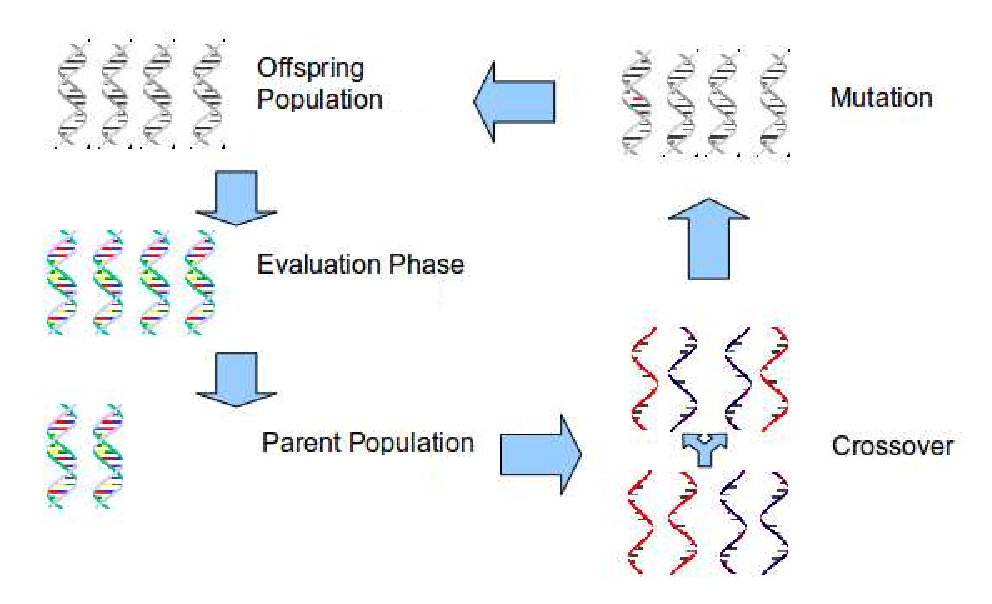
\includegraphics{EA.eps}}
\end{minipage}
\caption{Schematic representation of an EA. Each population is derived by the previous one via evolution operators, such as parent selection, crossover and mutation .} 
\label{EA}
\end{figure}


\section{Optimization problems - Definitions}
\label{OPt_def}
Any optimization problem with $M$ objectives (cast in vector $\vec{F}$) and $K$ constraints (cast in vector $\vec{C}$) can be formulated as:
\begin{align} 
   &min ~ \vec{F}(\vec{x})=(f_1(\vec{x}),f_1(\vec{x}),...,f_M(\vec{x}))\in \Re^{M} \nonumber \\
   &\mbox{subject to} ~ c_k(\vec{x})\leq d_k, ~~~~~ k =1,K
\label{OptimIN}
\end{align}
where $\vec{x}\in X \!\leq\! \Re^{N}$ is the design vector and $X$ the design space. If equality constraints $ c^*(x)=d^* $ are to be imposed, these can be transformed into inequality ones $ c(x)=\Vert c^*(x)-d^*\Vert \leq d $, where $ d \in \Re $ is an infinitessimally small number. If $M \!> \!1$, problem \ref{OptimIN} represents a multi-objective optimization (MOO) problem; in such a case, the notion of Pareto dominance \cite{Zitzler2000} is used to associate a scalar cost value to each individual, based on which an algorithm solving single-objective optimization (SOO) problems can be employed. In MOO problems, a single run of an EA is capable of delivering a Pareto front of non-dominated individuals, rather than a single "optimal" solution, standing for a compromise among the various objective functions. 

\subsection{Multi-Objective Optimization and EAs}
\label{MOOini}
In contrast to SOO, where the scalar cost function, which defines the survival of candidate solutions from generation to generation, is derived directly from the objective function, a MOO problem solver handles a vector of objectives. Therefore, in order to rely on the proposed for solving SOO problems EA, a technique to transform this vector to an appropriate scalar cost value is needed. In the literature, several techniques for handling this problem exist \cite{CoCo99,coe02,Miett99}. The most commonly used among them concatenate the $M$ objective functions into a scalar cost function, either by associating weights to each one of them or by accounting for the distance between the candidate solution and a user-defined ideal design or, even, using ranking techniques based on the notion of Pareto dominance (see below). In this PhD thesis, all MOO problems are handled using techniques relying on Pareto dominance criteria. Different implementations of Pareto dominance based techniques exist in the literature; among them, the most widely used ones are MOGA \footnote{Multi-objective Genetic Algorithm.} \cite{Fon93}, NPGA \footnote{Niched Pareto Genetic Algorithm.} \cite{horn94}, NSGA \footnote{Non-Dominated Sorting Genetic Algorithm.} \cite{Sri1995}, NSGA2 \cite{Deb00a}, SPEA \footnote{Strength Pareto Evolutionary Algorithm.}\cite{ZiTh98}, SPEA2 \cite{Zitz02,Zitz01}, PAES \footnote{Pareto Archived Evolution Strategy.} \cite{knowles99} and PESA \footnote{Pareto Envelope-based Selection Algorithm.} \cite{corne00}. The definition of Pareto dominance and Pareto optimality in minimization problems, which the aforementioned techniques rely on, follow:

\paragraph{Pareto Dominance:} Solution $\vec{x}_1$ dominates solution $\vec{x}_2$ ($\vec{x}_1\prec\vec{x}_2$) if and only if $\vec{F}(\vec{x}_1)$ is partially less than $\vec{F}(\vec{x}_2)$, i.e.
\begin{eqnarray}
    \vec{x}_1\prec\vec{x}_2 \Leftrightarrow (\forall i \in[1,M] :  f_i(\vec{x}_1) \leq f_i(\vec{x}_2))\wedge (\exists _i : f_i(\vec{x}_1) < f_i(\vec{x}_2))
   \label{pareto_eq} 
\end{eqnarray}

\paragraph{Pareto Optimality:} Solution  $\vec{x}_1 \in X$ is a Pareto optimal solution with respect to $X$ if and only if there is no $\vec{x} \in X$ that dominates $\vec{x}_1$, or 


\begin{eqnarray}
    \nexists\vec{x}:\vec{x}\prec\vec{x}_1, ~~~~ \vec{x},\vec{x}_1\in X \!\leq\! \Re^{N}
\end{eqnarray}
 
%\figuremacroW{Pareto2}{Pareto dominance}{Schematic representation of Pareto dominality. $\vec{x}_1$ is a Pareto optimal solution since it is not dominated by any other solution. Furthermore $\vec{x}_1$ itself dominates all individuals located in the grey box.}{0.5}

\begin{figure}[h!]
\begin{minipage}[b]{1\linewidth}
 \centering
 \resizebox*{!}{8 cm}{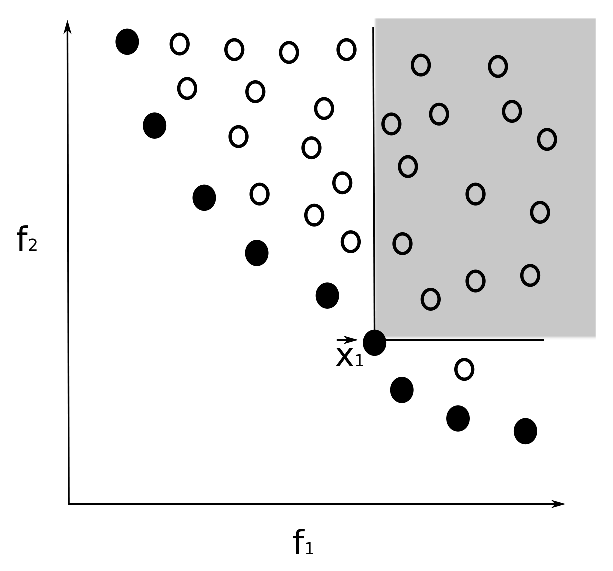
\includegraphics{Pareto2.eps}}
\end{minipage}
\caption{Schematic representation of Pareto dominance in a two-objective minimization problem ($min(f_1)$ and $min(f_2)$). $\vec{x}_1$ is a Pareto optimal solution since it is not dominated by any other solution. $\vec{x}_1$ dominates all individuals located in the grey box. All Pareto optimal solutions are noted as black circles.} 
\label{Pareto2}
\end{figure}


In fig. \ref{Pareto2}, a schematic representation of the Pareto optimality is presented. A minimization problem with two objective functions, $f_1$ and $f_2$, is considered. Black circles denote the front of non-dominated individuals whereas the empty circles denote dominated individuals. In the sake of clarity, the part of the objective space which is dominated by $\vec{x}_1$ is highlighted in grey. Individuals located in the grey area are dominated, at least, by $\vec{x}_1$. 

A detailed presentation of three techniques (SPEA,SPEA2 and NSGA2) used in this PhD thesis follows in section \ref{MOO}.

\subsection{Constrained Optimization and EAs}
\label{COPini}
In engineering, almost all optimization problems are subject to constraints which split the design space in feasible and infeasible regions. EAs may handle constraints through (a) the use of penalty functions \cite{Deb00,morales98}, by assigning greater chances to survive to individuals satisfying the constraints \cite{powell93}, (b) the conversion of constraints into objectives \cite{surry95,surry97} and/or (c) the use of correction operators \cite{mich94}. A detailed survey can be found in \cite{mich96,coello02}. In the present thesis, penalty functions are used as presented in section \ref{COP}. 

\section{The Evolutionary Algorithm SYstem (EASY)}
\label{EASY_def}
EASY is a generic optimization platform which implements the $(\mu,\lambda)EA$ \cite{phd_Giotis,phd_Karakasis,phd_Kampolis,EASYsite}. EASY has been developed by PCOpt/NTUA and the techniques proposed in this thesis have all been built on EASY. EASY supports MAEAs using on line trained metamodels, various forms of multi-level optimization as described in section \ref{EAintro}, distributed and asynchronous search; it is alsoGrid/Cluster-computing enabled, based on the DRMAA library. A detailed analysis of the implemented $(\mu,\lambda)EA$, considered as the background optimization method in this thesis, follows.  


\subsection{The $(\mu,\lambda)$EA}
\label{MLEA}
Each generation, denoted by the superscript $g$, of the $(\mu,\lambda)$EA is associated with three dynamically updated populations: the offspring $P_{\lambda}^g$ population with $\lambda$ offspring, the parent $P_{\mu}^g$ population containing $\mu$ parents and the elite $P_{e}^g$ population with $e$ elites. $P_{e}^g$ contains all or some of the currently best individuals. Depending on the design variables coding (binary, binary Gray or real), appropriate evolution operators are applied. 

The background $(\mu,\lambda)$ EA in use, \cite{phd_Giotis}, comprises the following steps:
\begin{itemize}
\item[]{\bf Step 1:}  (Initialization) $g=0$, $P_{e}^{g-1}=0$ and $P_{\mu}^g=0$. All $P_{\lambda}^g$  members are initialized using a pseudo-random number generator, in accordance to the user-defined lower and upper bounds for each design variable. A number of user defined individuals, such as existing sub-optimal designs for the same problem or optimal solutions to similar problems can optionally be included in the initial population. 
\item[]{\bf Step 2:}  (Evaluation) All individuals in $P_{\lambda}^g$ are evaluated using the problem-specific evaluation model. Below, this will also be referred to as ``exact evaluation model'' to clearly distinguish it from cheaper surrogate models. The evaluation step is, always, considered to be time-consuming and yields the vectors $\vec{F}(\vec{x}) \in \Re^{M} $ for each $\vec{x} \in P_{\lambda}^g$.
\item[]{\bf Step 3:}  (Cost assignment) For each $\vec{x} \in P_{\lambda}^g \cup P_{\mu}^g \cup P_{e}^{g-1}$, a scalar cost $\Phi(\vec{x})$ value is assigned based on $\vec{F}(\vec{x})$. In SOO, $\Phi(\vec{x})=F(\vec{x})$. In, MOO techniques the techniques presented in section \ref{MOO} are employed. 
\item[]{\bf Step 4:}  (Elite selection) The $e^*$ non-dominated (for MOO) or best (for SOO) individuals in $P_{\lambda}^g \cup P_{e}^{g-1}$ are selected to enter $P_e^g$. If $e^*\!>\!e$, a thinning operator \cite{phd_Giotis} can be applied to remove $e^*\!-\!e$ individuals.     
\item[]{\bf Step 5:}  (Elitism) A small number of elite individuals, selected, at random, from $P_e^g$, replace the worst members of $P_{\lambda}^g$.  
\item[]{\bf Step 6:}  (Parent selection) The new parent population $P_{\mu}^{g}$ is selected from $P_{\mu}^{g-1}$ and $P_{\lambda}^g$ by also taking into account the allowed maximum age  $k$ (measured in generations) of each individual. Symbolically, $P_{\mu}^{g}=S(P_{\mu}^{g-1},P_{\lambda}^g,k)$ 
\item[]{\bf Step 7:}  (Recombination and mutation) The next generation of the offspring population $P_{\lambda}^{g+1}$ is derived from 
$P_{\mu}^{g}$  by applying the recombination (or crossover) and mutation operators. Recombination $\mathcal{R}()$ is the process of combining the genotype of a number ($n$) of parents to create an offspring (see \ref{evOps}). The recombination operator is used $\lambda$ times, using differed sets of $n$ parents, randomly selected from $P_{\mu}^{g}$,  to create the $\lambda$ new offspring. Next step for the formation of $P_{\lambda}^{g+1}$ is the application of the mutation operator. Mutation $\mathcal{M}()$ is a process which with a small probability, randomly alters parts of the individual genotype. Symbolically, $P_{\lambda}^{g+1} = \mathcal{M}(\mathcal{R}(P_{\mu}^{g}))$ (see \ref{evOps}).
\item[]{\bf Step 8:}  (Stopping criterion) Unless any of the stopping criteria is met, return to $Step 2$.
\end{itemize}

The basic nomenclature of the ($\mu,\lambda$)EA is given in table \ref{GEA nomenclature}. 

\begin{table}[htdp]
\centering
\begin{tabular}{lr} 
\hline
\hline
Number of objectives & M\\
Number of design variables & N\\
Number of constraints   & K\\
\hline
Candidate solution, design vector   & $\vec{x}=(x_1,...,x_N)$\\
Objective function &$f_i(\vec{x})$ \\
Vector of objective values (if M$>\!1$)  &$\vec{F}=(f_1(\vec{x}),...,f_M(\vec{x}))$\\
Constraint function &$c_i(\vec{x})$ \\
Vector of constraint values  & $\vec{C}=(c_1(\vec{x}),...,c_K(\vec{x}))$\\
Scalar cost value (if M=1, $\Phi\!=\!f$) & $\Phi$ \\
\hline
Number of offspring &   $\lambda$ 			\\
Number of parents &  $\mu$ 				\\
Number of elites &  $e$			\\
Maximum allowed age &  $\kappa$			\\
Number of parents per offspring &  $\rho$			\\
\hline
\hline
\end{tabular}
\caption[GEA nomenclature]{Nomenclature of the ($\mu,\lambda$)EA.}
\label{GEA nomenclature} 
\end{table}


\subsubsection{Evolution operators}
\label{evOps}
The evolution operators employed in EASY are parent selection,  recombination, mutation and  elitism. These are further discussed below: 
   
\paragraph{Parent selection:}
The parent selection operator selects the members of $P_{\mu}^{g}$ from a set of individuals; in EASY, based on the sixth step of the  algorithm presented in section \ref{MLEA}, this set is the union of $P_{\mu}^{g-1}$ and $P_{\lambda}^g$. The most common parent selection techniques are: 
\begin{itemize}
\item[]{\bf a) Proportional selection.} Each member of $P_{\mu}^{g-1} \cup P_{\lambda}^g$ is given a probability to become a parent, which is inversely proportional to its cost value $\Phi$. Recall that a minimization problem is to be solved. The proportional selection is, practically, implemented via a roulette wheel algorithm. On the roulette wheel each and every set member is associated with a slot, the angular size of which quantifies its probability to become a parent. The roulette wheel is used $\mu$ times so as to create $\mu$ parents.  
\item[]{\bf b) Linear ranking.} In linear ranking, the $P_{\mu}^{g-1} \cup P_{\lambda}^g$ members are sorted according to their $\Phi$ values. The probability of each one of them to become a parent depends linearly on its position in the corresponding list and not on the $\Phi$ values themselves.
\item[]{\bf c) Probabilistic tournament selection.}
In probabilistic tournament selection \cite{goldberg1991}, a number of individuals are selected at random from the $P_{\mu}^{g-1} \cup P_{\lambda}^g$ set and with a user-defined, typically high, probability the best individual from this group is selected to become a parent, otherwise a randomly chosen, among the remaining individuals, becomes a parent. This process is repeated $\mu$ times so as to create $\mu$ parents. In tournament selection, the most important used-defined parameters are the tournament size i.e. how many individuals participate in each tournament and the probability that the best among them will be selected as parent. Typical values are: participation of $2$ or $3$ individuals in each tournament and $80\%$-$95\%$ probability to select the best among them.
\end{itemize}


\paragraph{Recombination:}
\label{RecombinationLabel}
Since the first appearance of EAs, there has been numerous discussions \cite{Schaffer87,Schaffer91,Navy92crossoveror} about the advantages of recombination used as an evolution operator in EAs. In general, the purpose of recombination is to increase the probability of an offspring to become fitter than its parent(s). Recombination schemes can be classified depending on the design variables coding. 

In EAs based on {\bf binary coding}, the recombination operator undertakes the exchange of pieces of the binary string encoding the design vector between the parents, in order to create an offspring. In EASY, the following types of binary coding recombination exist:
\begin{itemize}
\item[]{\bf a) One-point recombination.} 
In the one-point binary recombination, with $\rho$ parents per offspring, the binary string is divided into $\rho-1$ parts of equal length in binary digits. Then $\rho$ parents are selected at random from the $P_{\mu}^{g}$ set and $(\rho-1)$ pairs of parents are formed, with all of them including the first parent. If the first parent is denoted by 1, the $(\rho-1)$ pairs are: $(1,2),(1,3),...,(1,\rho)$. 
%The pairings take place serially between the lead parent (parent with higher $\Phi$) and the $i^{th} \in [1,\rho-1] $ one. 
For each one of the $(\rho-1)$ pairs, a random integer $\mathcal{X}$ determines the corresponding crossover point. The offspring is formed by combining the left part of the first parent string and the right part of the other parent, according to the aforementioned pairings. A three-parent example ($\rho=3$) is presented in fig \ref{1px}.
\begin{figure}[h!]
\begin{minipage}[b]{1.0\linewidth}
 \centering
 \resizebox*{11cm}{!}{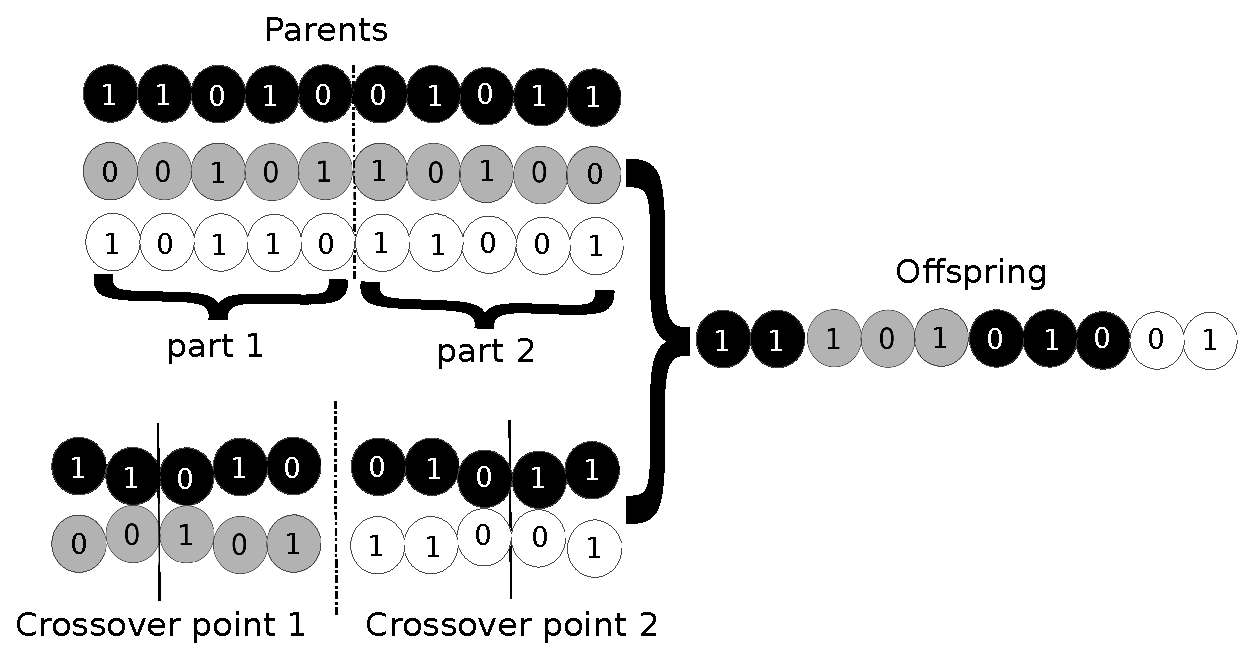
\includegraphics{onepointbinary.eps}}
\end{minipage}
\caption{One-point binary coding recombination with $\rho=3$. In this case, the chromosome is divided in two parts ($\rho-1 = 2$) and two vertical cuts are created at random.} 
\label{1px}
\end{figure}

\FloatBarrier
\item[]{\bf b) Two-point recombination}. This scheme is similar to its one-point counterpart, the only difference being that two crossover points $\mathcal{X}_1~\&~\mathcal{X}_2$ are used. A two-parent example is illustrated in fig \ref{2px}.

\begin{figure}[h!]
\begin{minipage}[b]{1.0\linewidth}
 \centering
 \resizebox*{11cm}{!}{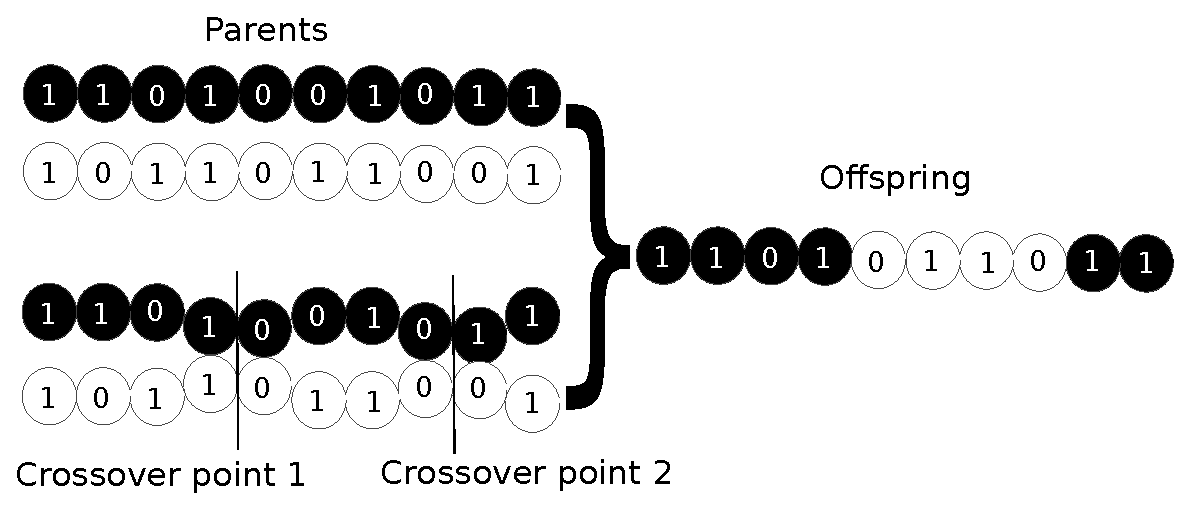
\includegraphics{twopointbinary.eps}}
\end{minipage}
\caption{Two-point binary coding recombination with $\rho=2$. In this simple case, the chromosome is handled as a whole ($\rho-1 = 1$) and two vertical cuts are created at random.} 
\label{2px}
\end{figure}

\FloatBarrier
\item[]{\bf c) One- or two-point recombination per design variable}. Here, the aforementioned one- and two-point recombination schemes are separately applied to the parts  of the binary string that correspond to each design variable.  
\end{itemize}
  
Using {\bf real coding} of the design variables $\vec{x}$, the recombination operator must be applied directly onto the real-valued design variables. In EASY, this is carried out as follows:  

\begin{itemize}
\FloatBarrier
\item[]{\bf a) One- or two-point recombination.} The one- and two-point recombination schemes, as described for binary coding, can be adapted to real coding by exchanging  pieces of the design vector $\vec{x}$ instead of pieces of binary strings. The randomly selected crossover variable is the only one to be affected by both parents according to a randomly generated weight $r$. A one-point, two-parent example is presented in fig \ref{1pxreal}.

\begin{figure}[h!]
\begin{minipage}[b]{1.0\linewidth}
 \centering
 \resizebox*{11cm}{!}{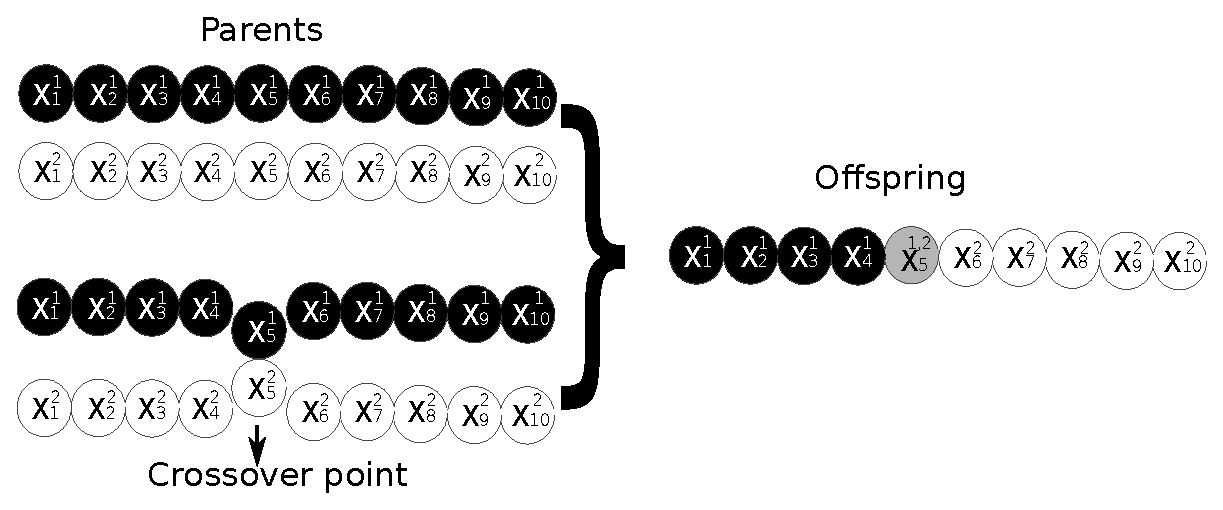
\includegraphics{pointreal.eps}}
\end{minipage}
\caption{One-point real coding recombination with $\rho=2$. The superscript denote the parent and the subscript the design variables. The crossover variable (e.g. $5$) is selected at random. In the offspring, this variable is given by  $x_5^{1,2}=x_5^{1}+r(x_5^{2}-x_5^{1})$, where $r$ is a random number, uniformly distributed in $[0,1]$ ($r \in U(0,1)$).    
} 
\label{1pxreal}
\end{figure}
 
\FloatBarrier 
\item[]{\bf b) Discrete recombination.} In discrete recombination with $\rho$ parents, each real-valued design variable in the offspring has $50\%$ probability to be copied either from the first parent $\vec{x}^1$ or any other  $\vec{x}^{random}$ randomly chosen among the $\rho-1$ remaining ones. A three-parent example is presented in fig \ref{disc}.

\begin{figure}[h!]
\begin{minipage}[b]{1.0\linewidth}
 \centering
 \resizebox*{11cm}{!}{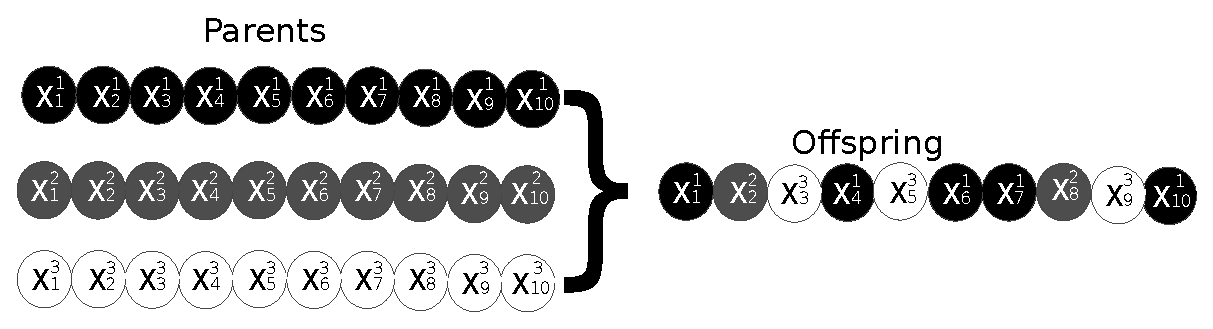
\includegraphics{discrete.eps}}
\end{minipage}
\caption{Discrete real coding recombination with $\rho=3$. $\vec{x^1}$ is the first parent.    
} 
\label{disc}
\end{figure}
    
\FloatBarrier    
\item[]{\bf c) Intermediate recombination}.  In intermediate recombination, each component of the offspring $\vec{x}$ is a linear combination of the first parent $\vec{x}^1$ and $\vec{x}^{random}$, which is randomly chosen among the $\rho-1$ remaining ones. Thus,
\begin{eqnarray}
\nonumber
\vec{x}=\vec{x}^1+r(\vec{x}^{random}-\vec{x}^1),~ r\in U[0,1]
\end{eqnarray}  
where $r \in U(0,1)$ means that $r$ is a random number, uniformly distributed in $[0,1]$. A different random number is generated for each design variable.

\FloatBarrier 
\item[]{\bf d) Simulated binary crossover}. The so-called simulated binary crossover (SBX) \cite{SBX1} aims at recreating the one-point binary recombination properties of (a) the average property \footnote{The average of the decoded variable values is the same
before and after the crossover operation.} and (b) the spread factor property\footnote{The spread factor ($\beta$) is defined as the ratio of the spread of offspring to that of parents. Contracting, expanding or stationary recombination correspond to $\beta <1$, $\beta >1$ or $\beta =1$ respectively. The spread factor property states that the occurrence of spread factor $\beta \approx 1$ is more likely than any other $\beta$ value. }\cite{SBX1}. The offspring $\vec{x}$ is generated based on the formulas
\begin{eqnarray}
	\vec{x}={\left\{ 
	\begin{array}{ll}
    \vec{\overline{x}} - \frac{\beta}{2} (\vec{x}^{random}-\vec{x}^1)~~,\mbox{if $r < 0.5$}\\
	\vec{\overline{x}} + \frac{\beta}{2} (\vec{x}^{random}-\vec{x}^1)~~,\mbox{if $r \geq 0.5$}
    \end{array} \right. }
    \label{sbxx}
\end{eqnarray}  
where $r\in U[0,1]$, $\vec{x}^1$ the first parent, $\vec{x}^{random}$ is randomly selected among the $\rho-1$ remaining parents, $\vec{\overline{x}}$ is the middle point between $\vec{x}^{1}$ and $\vec{x}^{random}$ and 
\begin{eqnarray}
	\beta={\left\{ 
	\begin{array}{ll}
    (2r)^{n}~~~~~~,\mbox{if $(r \leq 0.5)$}\\
	\left(\frac{1}{2r}\right)^{n+2}~~,\mbox{if $(r > 0.5)$}
    \end{array} \right. }
    \label{betasbx}
\end{eqnarray}

The probability distribution of $\beta$, given that $r\in U[0,1]$, can be plotted for various $n$ based on eq.\ref{betasbx} (fig.\ref{sbx};left). Based on the $\beta$ probability distribution and eq.\ref{sbxx}, the probability distribution of the offspring appearance on the design space as a function of $n$ can be plotted (fig.\ref{sbx};right for a 1D problem and fig.\ref{sbx2} for a 2D problem). In general, higher $n$ values increase the probability of $\beta \approx 1$, which in turn increases the probability of creating near-parent offspring (spread factor property). This together with the symmetrical offspring probability distribution with respect to $\vec{\overline{x}}$ (average property) shows that the "SBX" may in fact simulate the one point binary crossover.    

\begin{figure}[h!]
\begin{minipage}[b]{0.5\linewidth}
 \centering
 \resizebox*{7cm}{!}{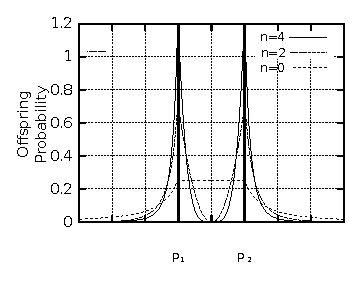
\includegraphics{SBXparents.eps}}
\end{minipage}
\begin{minipage}[b]{0.5\linewidth}
 \centering
 \resizebox*{7cm}{!}{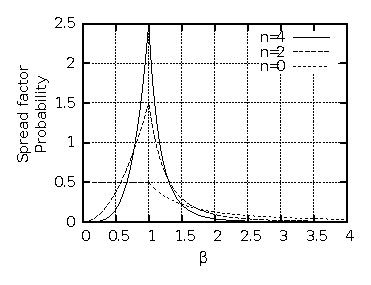
\includegraphics{SBX.eps}}
\end{minipage}
\caption{The offspring probability distribution of a 1D problem using SBX recombination with various $n$ is plotted as a function of the parents $P_1$ and $P_2$ (left). The corresponding probability distributions of $\beta$ are plotted on the right. Increasing $n$ leads to higher probability of $\beta \approx 1$.  }
\label{sbx}
\end{figure}

\begin{figure}[h!]
\begin{minipage}[b]{0.5\linewidth}
 \centering
 \resizebox*{7cm}{!}{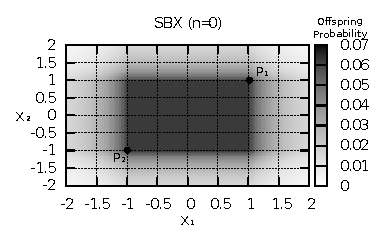
\includegraphics{SBX3dparents0.eps}}
\end{minipage}
\begin{minipage}[b]{0.5\linewidth}
 \centering
 \resizebox*{7cm}{!}{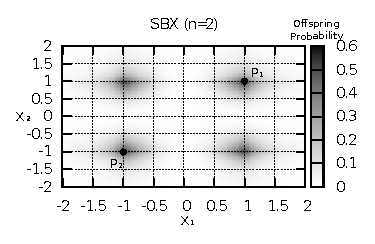
\includegraphics{SBX3dparents2.eps}}
\end{minipage}
\caption{The offspring probability distribution in a 2D optimization problem using SBX recombination for $n=0$ (left) and $n=2$ (right) is presented. The recombination uses two parents $P_1(1,1)$ and $P_2(-1,-1)$.}
\label{sbx2}
\end{figure}
\end{itemize}

\FloatBarrier   
\paragraph{Mutation:}
In an EA, the purpose of mutation is to introduce and preserve diversity in the population. Thus, mutation prevents the population from becoming homogenised prior to reaching the optimal solution, which would lead to slow or stagnated evolution. Mutation is applied to each offspring resulted from the recombination, subject to a small mutation probability $P_m$. Like recombination, mutation depends on whether binary or real coding is used.

In EAs based on {\bf binary coding}, the mutation is applied on each and every bit of the binary string. Each bit can be inverted (flip\footnote{Bit flip is a state switch, from 0 to 1, or vice-versa.}), with a probability $P_m$.      

\begin{figure}[h!]
\begin{minipage}[b]{1\linewidth}
 \centering
 \resizebox*{10cm}{!}{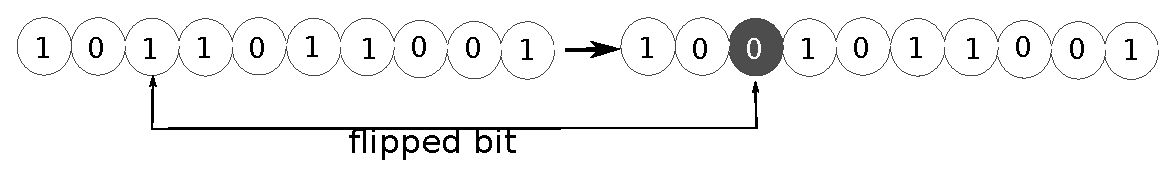
\includegraphics{mut.eps}}
\end{minipage}
\label{binarymut}
\end{figure}

\pagebreak
In {\bf real coded EAs},  mutation is applied on each real-valued component of $\vec{x}$, 

\begin{eqnarray}
	\vec{x}_m={\left\{ 
	\begin{array}{ll}
    \vec{x}~~~~~~~~~~,\mbox{if $(P_m > \vec{r})$}\\
	M(\vec{x},D)~,\mbox{if $(P_m \leq \vec{r})$}
    \end{array} \right. }
    \label{}
\end{eqnarray}
where $r\in U[0,1]$ and

\begin{eqnarray}
	M(\vec{x},D)={\left\{ 
	\begin{array}{ll}
    \vec{x}+D(g,\vec{U}-\vec{x})~,\mbox{if $(r_1 > 0.5)$}\\
	\vec{x}-D(g,\vec{x}-\vec{L})~,\mbox{if $(r_1 \leq r)$}
    \end{array} \right. }
    \label{}
\end{eqnarray}
where $r_1\in U[0,1]$, $\vec{U}$ and $\vec{L}$ are the vectors of upper and lower bounds of $\vec{x}$ accordingly and  

\begin{eqnarray}
   D(g,y) = y r_2 (1-g/g_{max})^{0.2}
\end{eqnarray}
where $g_{max}$ the number of maximum generations and $r_2\in U[0,1]$. If the maximum number of evaluations is determined by the termination criterion, then $g/g_{max}$ should be replaced with $Ev/Ev_{max}$ where $Ev$ is the evaluation count and $Ev_{max}$ the maximum allowed number of evaluations.  

%\begin{eqnarray}
%	\vec{\sigma}=\frac{min(\mid \vec{x}-\vec{UB}\mid,\mid \vec{x}- \vec{LB}\mid)}{3} * (1-\frac{g}{g_{max}})^p
%	\label{sigmamut} 
%\end{eqnarray}
%where $\vec{UB}$ and $\vec{LB}$ the vectors of upper and lower bounds for the design variables respectively. $g$ the current generation and $g_{max}$ the maximum allowed generations.$p \simeq 0.2$.

%The first part of the eq.\ref{sigmamut} ensures that the mutated individual will respect the design variable bounds and the second part reduces exponentially eith $p$ the magnitude of $\vec{\sigma}$ as the generations advance.

%\begin{figure}[h!]
%\begin{minipage}[b]{0.5\linewidth}
% \centering
% \resizebox*{7cm}{!}{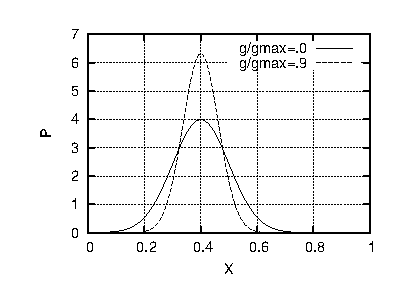
\includegraphics{Mut_1d.eps}}
%\end{minipage}
%\begin{minipage}[b]{0.5\linewidth}
% \centering
% \resizebox*{8cm}{!}{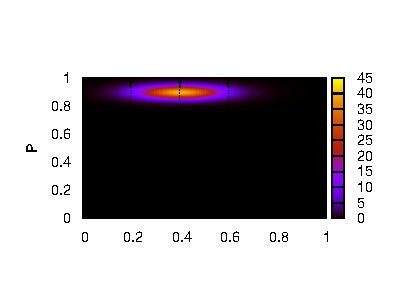
\includegraphics{Mut_2d.eps}}
%\end{minipage}
%\label{realmut}
%\caption{Examples of mutant probability distributions for one design variable left $x=0.4$ and two design variable right $\vec{x}=(0.4,0.9)$. For both cases $\vec{LB}=0$ and $\vec{UB}=1$.}
%\end{figure}

\paragraph{Elitism:}
In EAs, the purpose of elitism is to guarantee a monotonously improving course of evolution \cite{Back1996}. In EASY, a separate population $P_e^g$ is maintained, updated accordingly in each generation (see step 4 of the ($\mu,\lambda$)EA in section \ref{MLEA}). Elitism takes place when a number of user-specified elite individuals replace the worst members of the offspring population $P^g_{\lambda}$ before the application of the parent selection operator.
  
\subsection{Solving MOO Problems with EASY}
\label{MOO}
As mentioned in \ref{MOOini}, in MOO problems, a technique that transforms $\vec{F}$ into a scalar cost function $\Phi$ is required. Symbolically,

\begin{eqnarray}
    \Phi(\vec{x})=\Phi(\vec{F}(\vec{x})) :\Re ^M \rightarrow \Re ^1 
	\label{MOOeq}
\end{eqnarray}
The SPEA, SPEA2 and NSGA2 techniques, which are available in EASY, are presented below:

\paragraph{SPEA:}
SPEA was proposed by Zitzler and Thiele \cite{ZiTh98} in 1998 as a MOO cost assignment technique based on Pareto dominance. In SPEA, the computation of $\Phi(\vec{x})$ takes place in two steps, namely:
\begin{itemize}

\item[]{\bf Step 1:}  (Strength calculation) The strength of each member of the population $P=P_{\lambda}^g \cup P_{\mu}^g \cup P_{e}^{g-1}$ is computed. The strength of the individual $i$ ($S_i$) is defined as the sum of the population members that are dominated  by $i$ divided by the total number of the individuals in the population,  

\begin{eqnarray}
	S_i = \frac{\sum(j : j \in P \wedge i \prec j)} {\sum P}, ~~ \forall i \in P =P_{\lambda}^g \cup P_{\mu}^g \cup P_{e}^{g-1}  
\end{eqnarray}

\item[]{\bf Step 2:}  (Cost calculation) The cost value $\Phi$ for each population member is calculated as the sum of strengths of the population members that dominate it,

\begin{eqnarray}
	\Phi_i = \sum _{j \in P \wedge i \prec j}(S_j)
\end{eqnarray}
\end{itemize}
  
 
\paragraph{SPEA2:}
SPEA2 \cite{Zitz02,Zitz01} is an enhanced variant of SPEA which additionally incorporates density information. A nearest neighbour density estimation technique which allows a more precise guidance of the search process is incorporated, improving, in comparison with the SPEA, the distribution of the individuals on the resulting Pareto front. 

The SPEA2 algorithm performs three steps to compute $\Phi$. These steps are:

\begin{itemize}
\item[]{\bf Step 1:}  (Strength calculation) As in SPEA.

\item[]{\bf Step 2:}  (Density calculation) For each member of the population the density metric $D_i$ is calculated  as a function of its distance from its closest neighbour in the objective space $d_i$,

\begin{eqnarray}
	D_i = \frac{1} {d_i+2} 
\end{eqnarray}
where
\begin{eqnarray}
	\nonumber
	d_i= min (\parallel \vec{F_i} - \vec{F_k} \parallel), ~ k \in P  
\end{eqnarray}


\item[]{\bf Step 3:}  (Cost calculation) The cost values for all population members are calculated as the sum of the raw cost $R_i$ and the density metric,

\begin{eqnarray}
	\Phi_i = R_i+D_i
\label{SPEAIIeq}
\end{eqnarray}
Here, $R_i$ is the sum of the individual strengths of the population members that dominate it,
  
\begin{eqnarray}
	\nonumber
	R_i=\sum _{j \in P \wedge i \prec j}(S_j)  
\end{eqnarray}  
\end{itemize}

\paragraph{NSGA2:} 
NSGA2 \cite{Deb00a} is an improved version of NSGA \cite{Sri1995} addressing the high computational complexity of non-dominated sorting, the lack of elitism and the need for specifying the sharing parameter of the initial algorithm. A modified version of NSGA2 is available in EASY. The NSGAII as proposed in \cite{Deb00a} instead of calculating $\Phi$ values, relies upon the sorting of the individuals according to Pareto dominance and density criteria. The modified variant of NSGA2 used in this PhD thesis, which calculates $\Phi$ values, includes the following steps:    


\begin{itemize}
\item[]{\bf Step 1:}  (Front ranking) All members of the population are classified in fronts with decreasing Pareto dominance.  
\begin{itemize}
\item[]{\bf Step 1-a:}  (Initialisation) Initialisation of front number $i=0$ and auxiliary set $S=P_{\lambda}^g \cup P_{\mu}^g \cup P_{e}^{g-1}$.

\item[]{\bf Step 1-b:}  (Find non-dominated members of $S$) Locate the non-dominated members of $S$ and copy them to $\mathcal{F}_i$. 

\item[]{\bf Step 1-c:}  (Update) Update $S=S-\mathcal{F}_i$ and $i=i+1$. if $S>0$ go to Step 1-b else, set the number of fronts $N_F$ equal to $i-1$ and go to Step 2.
\end{itemize}
\item[]{\bf Step 2:}  (Density calculation) For each member $j \in \mathcal{F}_i$, the density metric $d_j$, which is equal to the average side-length of the cuboid defined by its neighbouring individuals in $\mathcal{F}_i$, is calculated. This procedure is repeated for all fronts $i$, so as all individuals are given a density metric value.

\item[]{\bf Step 3:}  (Cost calculation) Based on the density metric (calculated in Step 2) and the front $i$ (calculated at Step 1) that each individual belongs to, a scalar $\Phi$ is assigned to each individual as follows,
\begin{itemize}
\item[]{\bf Step 3-a:}  (Initialization) Initialise $i=0$ and $\Phi_b=1.0$.
\item[]{\bf Step 3-b:}  ($\Phi$ calculation) For each member $j \in \mathcal{F}_i$, $\Phi$ is calculated as

\begin{eqnarray}
	\nonumber
	\Phi_j= \Phi_b(1+\frac{d_{max}-d_j}{d_{max}}) 
\end{eqnarray} 
where $d_{max}$ the maximum $d_k$ $\forall k \in \mathcal{F}_i$   
\item[]{\bf Step 3-c:}  (Update) Update $\Phi_b=1.1max(\Phi_j)$ and $i=i+1$. If $i \leq N_F$ go to Step 3-b, otherwise stop. 
\end{itemize}
\end{itemize}

\subsection{Constraints handling in EASY}
\label{COP}
In EASY, penalty functions are used to handle constraint optimization problems (COP), see section \ref{OPt_def}. Penalty terms, proportional to the magnitude of the constraint violation, are added to the cost function. According to eq.\ref{penal2}, for each constraint, a ``nominal threshold'' $d_k$ is defined as the maximum possible constraint function value as described by the optimization problem. Furthermore, a ``relaxed'' threshold $d_k^* > d_k$ is introduced. Once an individual violates the relaxed threshold of one of the constraints ($c_k>d_k^*$), death penalty ($\Phi = \infty$) is given to it. If the individual violates one or more of the constraints ($d_k<c_k<d_k^*$) but none of the relaxed threshold values, its cost value $\Phi$ is penalized as follows:

\begin{eqnarray}
	\Phi(\vec{x})=\Phi(\vec{x})+ \prod _{k=1}^K{\left\{ 				\begin{array}{ll}
    exp(a_k\frac{c_k(x)-d_k}{d_k^* -d_k}) & ~~,c_k(x)>d_k\\
    1 & ~~,c_k(x)\leq d_k\end{array} \right. }
    \label{penal2}
\end{eqnarray}  
where the user-defined set of coefficient values in $\vec{a}$ control the penalization intensity.

%\begin{figure}[h!]
%\begin{minipage}[b]{1.0\linewidth}
% \centering
% \resizebox*{10cm}{!}{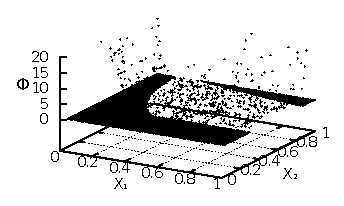
\includegraphics{fit_new.eps}}
%\end{minipage}
%\caption{$\Phi$ plot for 1000 randomly chosen individuals over the 2d design space of a two-objective constrained optimization problem (fig.\ref{case}) using the proposed penalization formulation (eq.\ref{penal2}).}
%\label{fit2}
%\end{figure}
 

\subsection{Metamodel-Assisted Evolutionary Algorithm (MAEA)}
\label{MAEApar}
Due to the involvement of costly evaluation models (such as CFD software to numerically predict flows in or around complex 3D geometries), solving engineering optimization problems using EAs may become very computationally demanding. The extensive, smart use of low-cost surrogate evaluation models (often referred to as "metamodels") during the optimization decreases substantially the number of calls to the computationally expensive, problem-specific evaluation code (CFD). This makes EAs a viable tool that can routinely be used to solve large-scale industrial optimization problems, in affordable wall clock time. Literature surveys on the use of metamodels within EAs can be found in papers \cite{LTT_2_020,Jin2002,LTT_2_027,EBNK} or books \cite{KEANEbook}.


Polynomial regression, artificial neural networks, Gaussian processes etc. have all been used as metamodels. The existing MAEAs differ since they apply different interactions between the metamodel and the problem-specific evaluation models. Hereafter, all of them will be referred to as MAEAs. In this thesis, on-line trained metamodels are in use \cite{LTT_2_018,LTT_2_020,LTT_2_029}. 
 
In on-line trained metamodels, for all but the first few generations, the metamodels are used to pre-evaluate the current population. Based on the outcome of approximate pre-evaluations (Inexact Pre-Evaluations, IPE), the few most promising individuals are identified and these solely undergo evaluation with the problem-specific evaluation model to compute their ``exact'' (high-fidelity) objective function value(s), before proceeding to the next generation. The $(\mu,\lambda)$ MAEAis sketched in fig.~\ref{MAEA}.


\begin{figure}[h!]
\centering
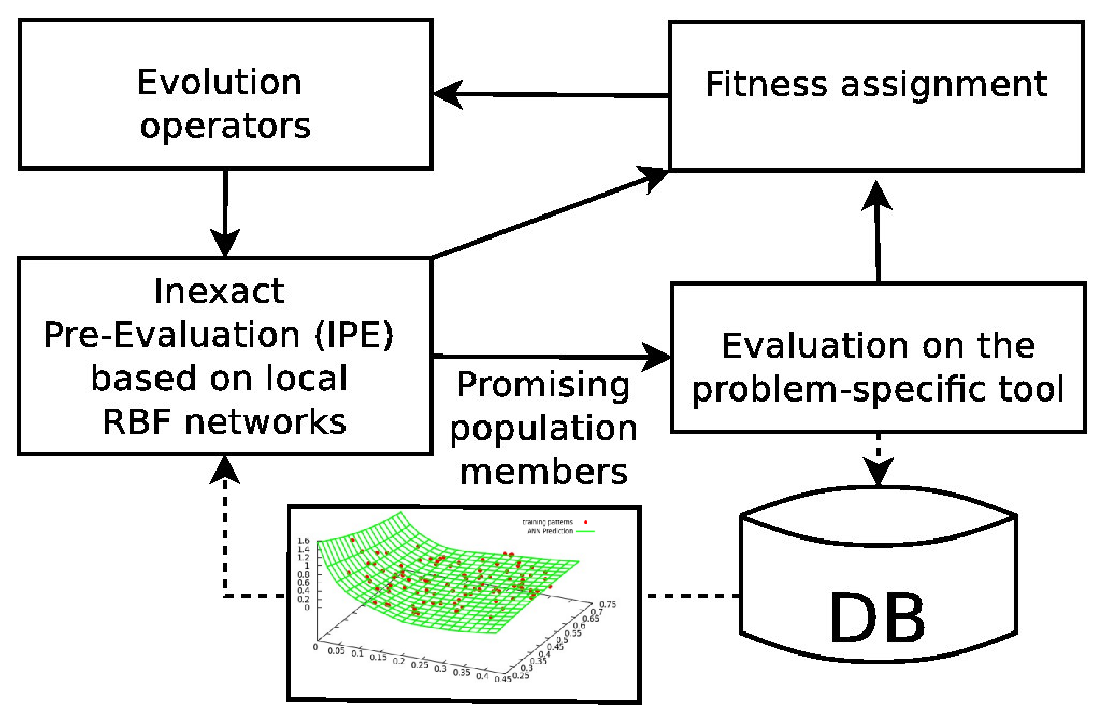
\includegraphics[width=90mm]{MAEA.eps} 
\caption{The $(\mu,\lambda)$MAEA using on-line trained metamodels. The loop corresponds to a single EA generation. The so-called Inexact Pre-Evaluation (IPE) phase, within the EA--based search, is described in \cite{LTT_2_018,LTT_2_020,LTT_2_029}. }
\label{MAEA}
\end{figure}


\paragraph{Radial Basis Function (RBF) networks}
In this PhD thesis, RBF networks are used as metamodels, though the new methods proposed in the next chapters could be combined with any other type of metamodels. RBF networks are artificial neural networks (ANNs) with three neuron layers, (input,hidden and output) as shown in fig.\ref{rbf1} \cite{Haykin}. Signals propagate through the network in the forward direction, from the input to the output layer, by performing a nonlinear mapping (eq.\ref{RBFa}) followed by a linear one. The latter is related to the weight coefficients $w_l$ that must be computed during the training on a number of available patterns. An RBF network to be used within a MAEA should have $N$ input units, i.e. as many as the  design variables. The hidden layer includes $L$ nodes, associated with the so–called RBF centers $c^l$. At each hidden neuron, a nonlinear mapping of the input signals to a single value is carried out using the radial-basis activation function $G:\Re^N \rightarrow \Re$, acting on the distance of input $\vec{x}$ (eq.\ref{RBFa}) from the corresponding center $\vec{c^l} \in \Re^N$.  In the current thesis, the Gaussian activation: 

\begin{eqnarray}
	G(u,r)=exp(\frac{-u^2}{r^2})
	\label{RBFa}
\end{eqnarray}  
where $u=\Vert x-c^l \Vert_2$ the distance from the corresponding $l^{th}$ RBF center, is used.

\begin{figure}[h!]
\centering
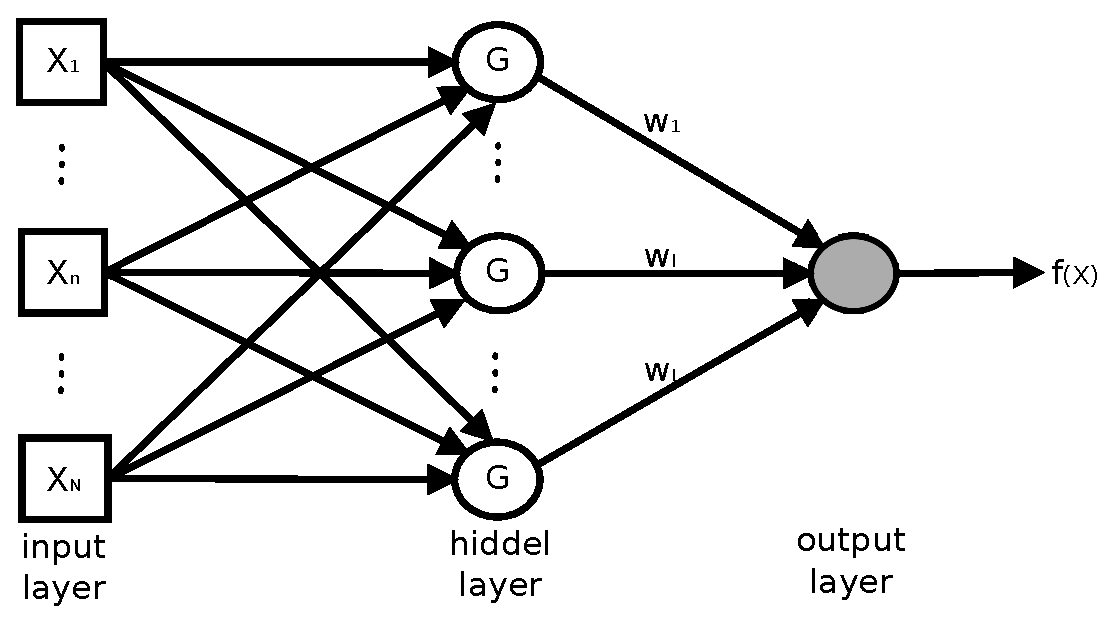
\includegraphics[width=90mm]{RBF.eps} 
\caption{Radial basis function (RBF) network.}
\label{rbf1}
\end{figure}
The radii or widths r values may considerably affect the prediction abilities of the network; these are computed using heuristics \cite{Haykin}. The output layer includes as many nodes as the expected responses of the network. The single response we are dealing with is expressed by the sum of the weighted output signals from the hidden neurons, as follows:             
\begin{eqnarray}
	f(x)=\sum _1^K w_i*G(u(x_i),r)
\label{response}
\end{eqnarray}  

If the number of hidden nodes ($K$) is equal to the number of training patterns ($T$), the choice of the $RBF$ centers is straightforward, i.e.
$\vec{c}^{(t)}\!\equiv\!\vec{x}^{(t)}$, $t\!\in\![1,T]$, ensuring
that the $T$ samples are exactly interpolated. 
In this case, the network training is reduced to the solution of a $T\!\times\!T$ symmetric linear system of equations, as follows:
%
\begin{equation}
    \sum_{t=1}^{T} w_t G(\|\vec{x}^{(t)}-\vec{c}^{(t)}\|_2)=
    \zeta^{(t)}
    \nonumber
\end{equation}

A common way to increase the network's generalization \cite{Pog1990, Tik76, Tik95} is by using a smaller number of, appropriately selected, hidden nodes than the training patterns, i.e. selecting $K\!<\!T$. 
In this case, the selection of the $RBF$ centers is not straightforward, as in the aforementioned case, and is of great importance since 
it strongly affects the prediction ability of the network. 
In \cite{LTT_2_029}, a selection scheme for the $RBF$ centers based on 
self-organizing maps ($SOMs$, \cite{Fri94a, Hayk1999}) was proposed. 
This practically comprises a two level learning scheme, namely the unsupervised and the supervised ones.
During the unsupervised learning, $SOMs$ (through their standard processes: 
competition, cooperation and adaptation) classify the training 
patterns into $K$ clusters.  
Each cluster gives a single $RBF$ center $\vec{c}^{(k)}$, considered to be representative of the cluster as a hole. The corresponding radius $r_k$ is computed using heuristics based on distances between the centers, \cite{Karay1997, LTT_2_029, Hayk1999, BenArc02}.
During the supervised learning, the synaptic weights are computed by minimizing the approximation error of the $RBF$ network over the training set, while considering smoothness requirements.
%
%\begin{figure}
%    \centering
%    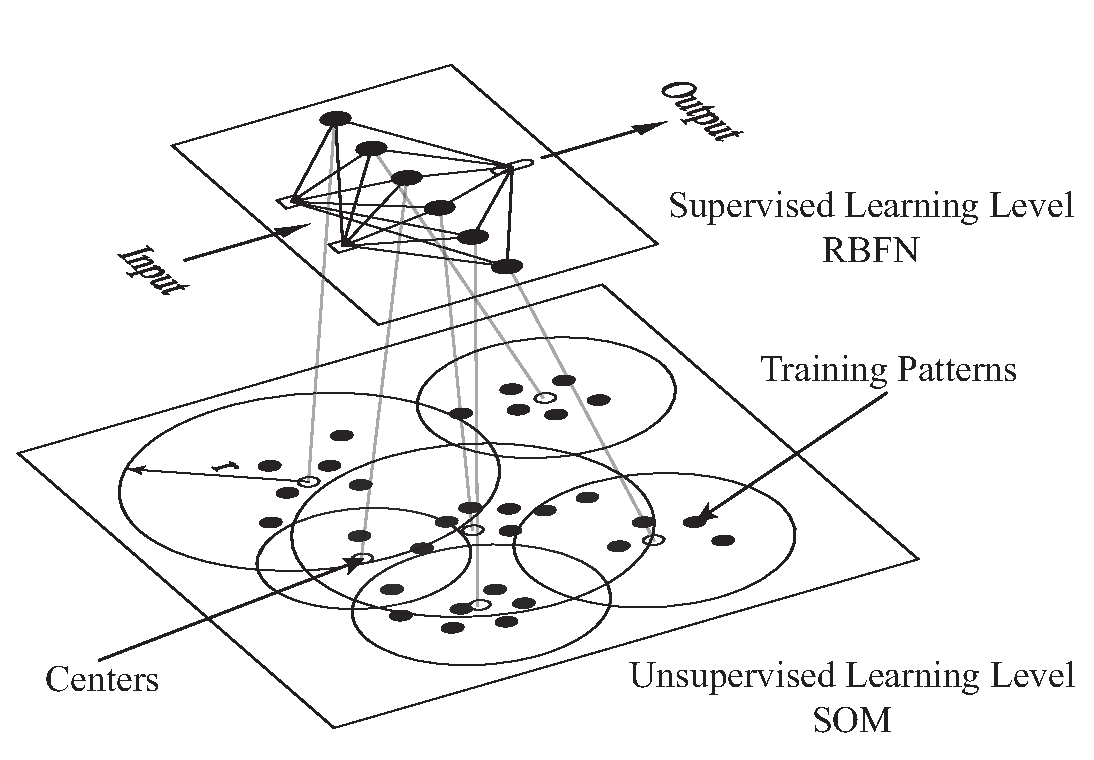
\includegraphics[scale=0.6]{rbf-som.eps}
%    \caption{The two phases of an \RBF\ network training based on \SOMs:
%            (a) self-organized positioning of the \RBF\ centers (unsupervised 
%            learning) and (b) computation of the synaptic weights (supervised
%            learning.}
%    \label{f:rbfn-som}
%\end{figure}


The so--called \textit{Importance Factors} ($IFs$), as proposed by Giotis A.P et al. in \cite{LTT_2_018}, can improve the prediction ability of the $RBF$ network. Incorporating $N$ extra coefficients ($I_n, n\!=\!1,N$), the importance of each design parameter on the network response is quantified and exploited in order to increase the overall $RBFn$ prediction quality. High $I_n$ values indicate high sensitivity of the objective function in the vicinity of the design point under consideration with respect to the $n$-th input variable. The $IFs$ are computed by the $RBF$ network as a by-product of the training process and are used to improve the quality of the networks' output. 
In detail, each time an improved solution is computed by the $EA$ (index $b$, which stands for the current best), a local $RBF$ network is built and $N$ partial derivatives $\partial o^{(b)} / \partial x_{n}$ are computed using the network's closed-form expressions; by doing so, $\partial o^{(b)} / \partial x_{n}$ are the exact derivatives of an approximate function. 
Based on these derivatives, a weighted norm is introduced and used instead of the standard one (i.e. instead of eq. \ref{response}), as follows
%
\begin{equation}\label{e:IFcomp}
    \left\|\vec x^{(t)}-\vec c^{(k)}\right\|_{wei} =
    \sqrt{  \sum_{n=1}^N I_n\left(x_n^{(t)}-c_n^{(k)}\right)^2  }
	\mbox{,~where~~~~}
    I_n = { {\left|  {\partial o^{(b)}} \over {\partial x_n} \right|} 
          \over 
  { \sum_{i=1}^{N} \left| {\partial o^{(b)}} \over {\partial x_i} \right| } }
\end{equation}


\subsubsection{Inexact Pre--Evaluation algorithm}


The algorithm starts as a conventional $(\mu, \lambda)EA$ (by, exclusively, making use of the exact evaluation model) for the few starting generations until a user--defined minimum number of previously evaluated individuals enter the $DB$. 
Then, the $IPE$ phase starts and, in subsequent generations, instead of evaluating the offspring population on the costly, problem--specific model, the following actions are taken:
\newcommand{\apprx}[1]{\tilde{#1}}
\begin{itemize}
\item[]{\bf Inexact evaluation:}
For each offspring, $\vec{x}\!\in\!P_{\lambda,g}$, the objective function values $\apprx{\vec{F}}(\vec{x})$, are approximated using a local metamodel trained on a small number of data selected from the $DB$. 
%
\item[]{\bf Screening:}
%>>>>
Based on the $\apprx{\vec{F}}(\vec{x})$ values, a provisional
$\Phi$ value (denoted by $\apprx{\Phi}$) is assigned to each
offspring.
%>>>>
\item[]{\bf Exact evaluation:}
%>>>>
For all $\vec{x}\!\in\!P_{e}$, the exact objective function values $\vec{F}(\vec{x})$ are computed and stored in the $DB$. 
Practically, this step, determines the $CPU$ cost of each generation.
%...................
\end{itemize}


\subsection{Hierarchical Evolutionary Algorithms}
Typically, in engineering design, a number of models with different fidelity and cost (computational and/or economical) might be available and these can be used in different steps of the design procedure (fig.\ref{HMAEA} right). Relatively fast low fidelity models are used in the initial stages of the design in order to efficiently scan the design space allowing a big number of relatively low cost calls the the evaluation model. High fidelity models, expensive (computational, high computational demand, and/or economical, licensed software or laboratory time,) are used for the latter steps of design for fine-tuning offering detailed and reliable information about each candidate solution. Furthermore, different types of parametrization offering either course or detailed shape representations are also available and in use. A fairly course shape representations is used during the initial steps of the design procedure in order to locate the rough shape of the optimal geometry and during the design procedure the detail of the shape parameterization increases as the designer wishes to obtain more detail control over his design.

An example of this kind of design procedure, as used in hydro-turbine-industry (ANDRITZ HYDRO), is shown in fig.\ref{HMAEA} right. As a fast but low fidelity flow predicting model an Euler solver is used. Using the Euler solver a fairly big number of candidate geometries are analysed (black arrows denote the number of design cycles performed) as soon as the designer locates a design that fulfils his criteria he proceeds with evaluating the design using the high fidelity model in this case a Navier-Stokes solver.  Typically a lot less evaluations (and less design cycles) are made using the high fidelity model due to mainly its computational but also economical (licence) cost.  During this design procedure the designer often falls buck from using the high to using the low fatality model (as the external design cycles (black arrows) denotes) this implies that the designer has observed a pattern concerning the deferences between the high and low fidelity models and uses it to update his criteria concerning the lower fidelity model design cycles. The simplest example of that is the observation that the low fidelity model overestimates the velocities near the walls in comparison with the high fidelity one, so the designer could continue to design using the lower model but looking for a design that yields higher (magnitude depending on the difference between the two models) velocities near the walls. As the total number of design cycles increases the shape representation complexity also increases (additional control points) giving the designer grater flexibility/control over his design.      


\begin{figure}[h!]
\begin{minipage}[b]{1.0\linewidth}
 \centering
 \resizebox*{13cm}{!}{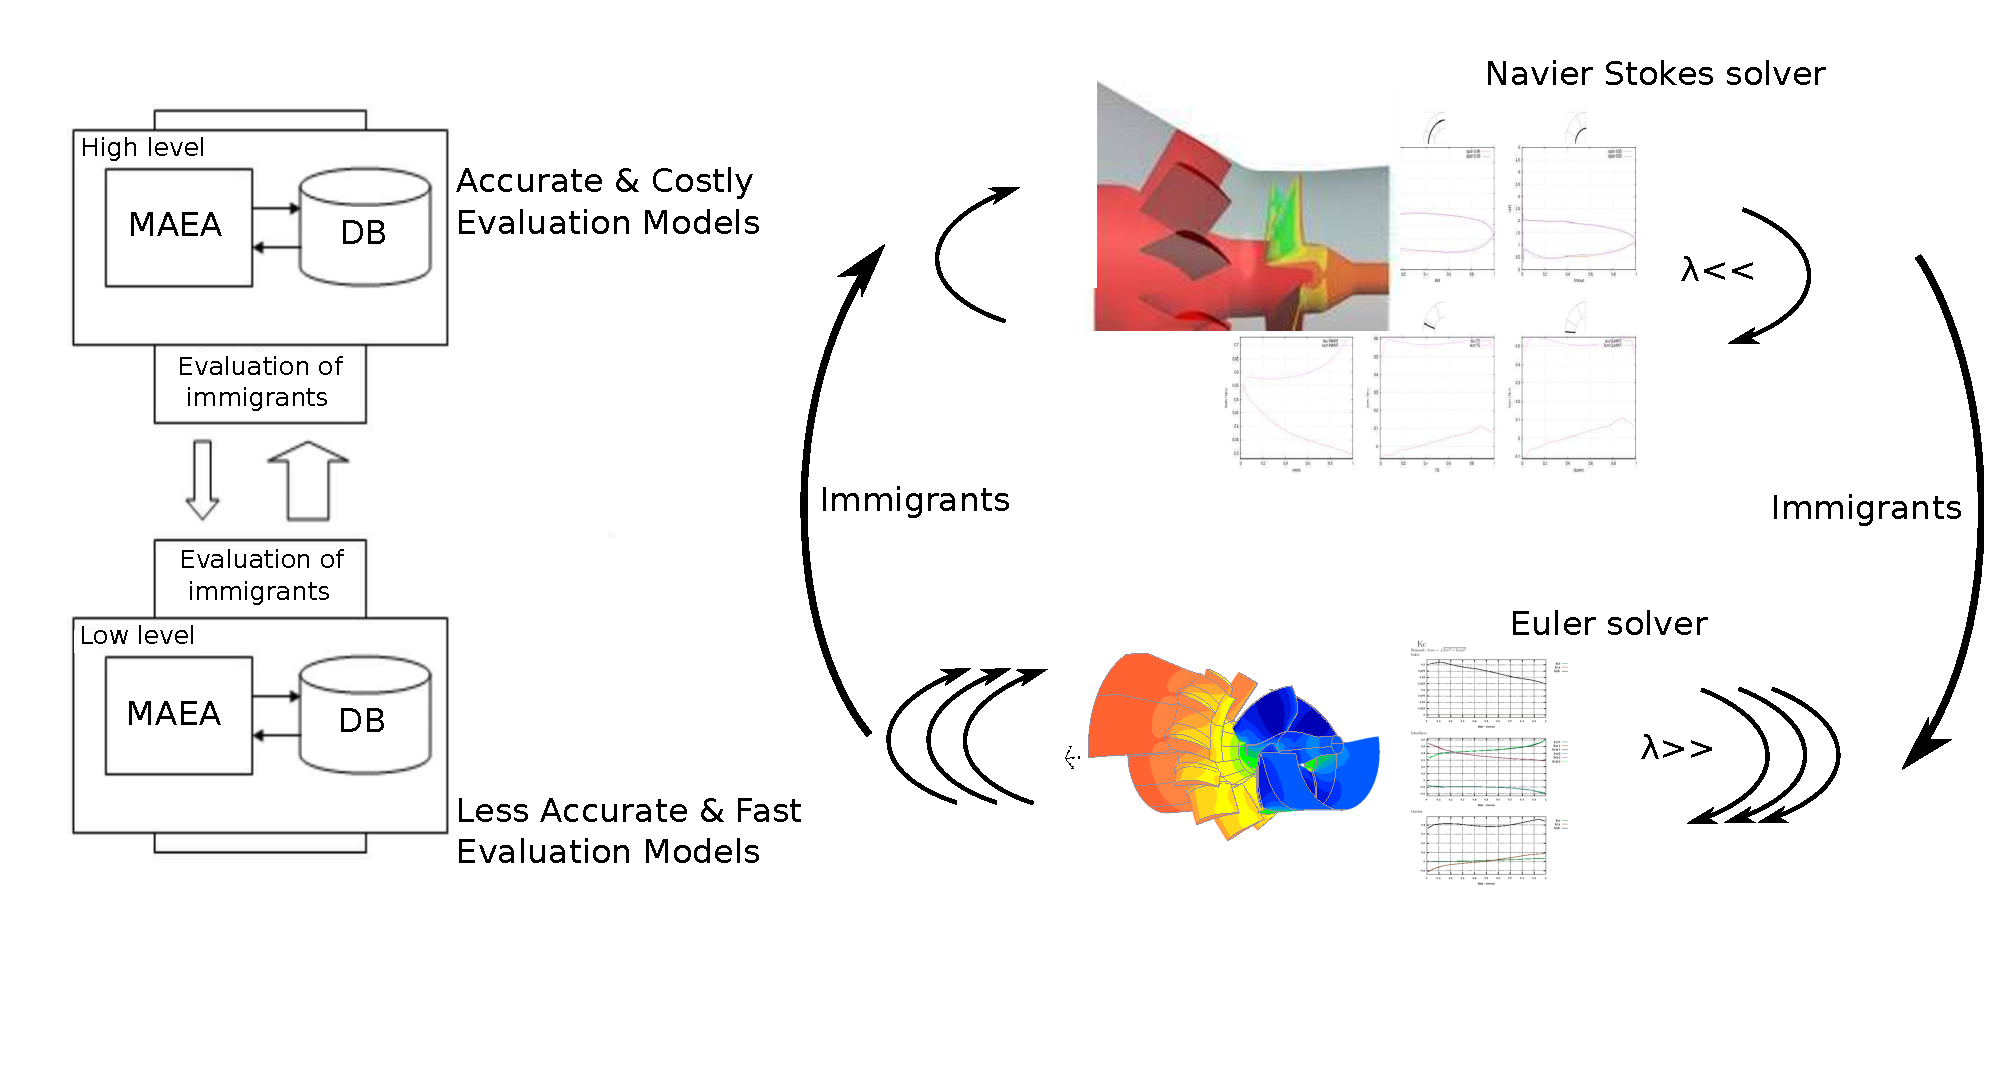
\includegraphics{handmade.eps}}
\end{minipage}
\caption{Left: schematic representation of a two-level HMAEA (Hierarchical metamodel-assisted EA). The high level is associated with the expensive and accurate model and the lower level with the cheap and thus less-accurate one. Communication between the two level is possible in both directions including re-evaluation with the receiving levels evaluation tool. Right: Example of the manual design procedure, as used in hydro-turbine-industry (ANDRITZ HYDRO).}
\label{HMAEA}
\end{figure} 
 
In order to exploit the availability of multiple models, multiple representations and multiple search algorithms (since this is an automated design procedure) Hierarchical EAs (HEA) were devised \cite{Herr1999, Sefr2000, Desid2003, LTT_2_031, LTT_3_092, LTT_2_036,
LTT_2_044, LTT_2_048, LTT_4_05}. HEA are enhanced EA variants which utilise a number of evolution Levels, each level assigned a different evaluation model (fig.\ref{HMAEA} left) parameterization scheme or search algorithm. This multilevel search mechanism splits the computational burden among the levels. On the lower levels, a low cost exploration of the search space is carried out through global search methods (EAs), less demanding or less accurate evaluation models or by even using reduced design variable sets, etc. On the other hand the higher levels undertake the fine-tuning part of the design procedure through detailed parameterization, more accurate evaluation models and/or stochastic or deterministic search methods. These levels mainly serve to refine immigrants from the lower levels. Intercommunication and two-way migrations of individuals between adjacent levels are available. The number of levels, the frequency of migration and the number of immigrants are user-defined parameters.

To sum up, the HEAs mechanisms can be categorized in three main types, that of course can be combined in any resulting schemes, namely the hierarchical evaluation,  search and parameterization (fig. \ref{allheas}). In hierarchical evaluation schemes the availability of evaluation models with different cost and fidelity is exploited. In  the hierarchical search, different search algorithms are optimally combined. In hierarchical parameterization, both rough and detailed shape representations can be combined in a single automated design procedure. 

\begin{figure}[h!]
    \centering
    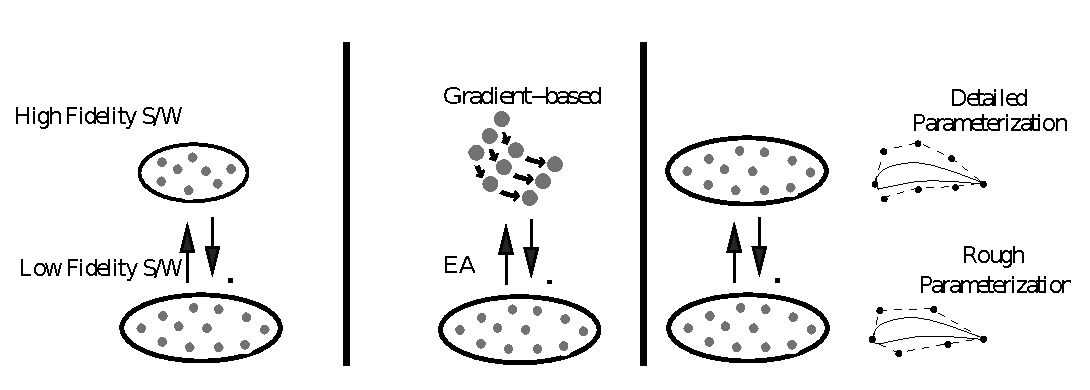
\includegraphics[scale=0.8]{multimodes.eps}
% ------------------------------------------------
    $\mbox{Hierarchical Evaluation~~~~~Hierarchical Search~~~~~~Hierarchical Parameterization}$
%   $\mbox{Hierarchical}~~~~~~~~~~~~~~~~
%    \mbox{Hierarchical}~~~~~~~~~~~~~~~~~~~~
%    \mbox{Hierarchical}$
%   \\
%   $~~~\mbox{ Evaluation }~~~~~~~~~~~~~~~~~~
%    \mbox{   Search   }~~~~~~~~~~~~~~~~~~~
%    \mbox{Parameterization}$
% ------------------------------------------------
    \caption{$HEAs$. Schematic representation of the three
            hierarchical schemes. Left: schematic representation of the hierarchical evaluation scheme. Middle: schematic representation of the hierarchical search scheme. Right: schematic representation of the hierarchical parametrization scheme. All this types can be combined or used separately at will utilizing two or more levels.}
    \label{allheas}
\end{figure}      
% ---------------------------------------------------------------------------
% ----------------------- end of thesis sub-document ------------------------
% ---------------------------------------------------------------------------